\documentclass[a4paper,12pt]{article}

\usepackage{../usfdvl}


\title{Worksheet 2}
\SetDocumentFooter{}{}


\begin{document}

\maketitle


\vspace{5pt}
\section{Ground Rules}

\myparagraph{This assignment is intended to be done alone. You may ask others for high-level help. However, the answer must be yours.}

\vspace{5pt}
\section{Assignment}

\begin{enumerate}
\item For the following polygon:
\begin{itemize}
\item Draw all possible edges between non-adjacent vertices. 
\item Denote those segments which are diagonals and those which are not. 
\item For non-diagonal segments, state the reason they are not considered diagonal. 
\end{itemize}

\begin{center}
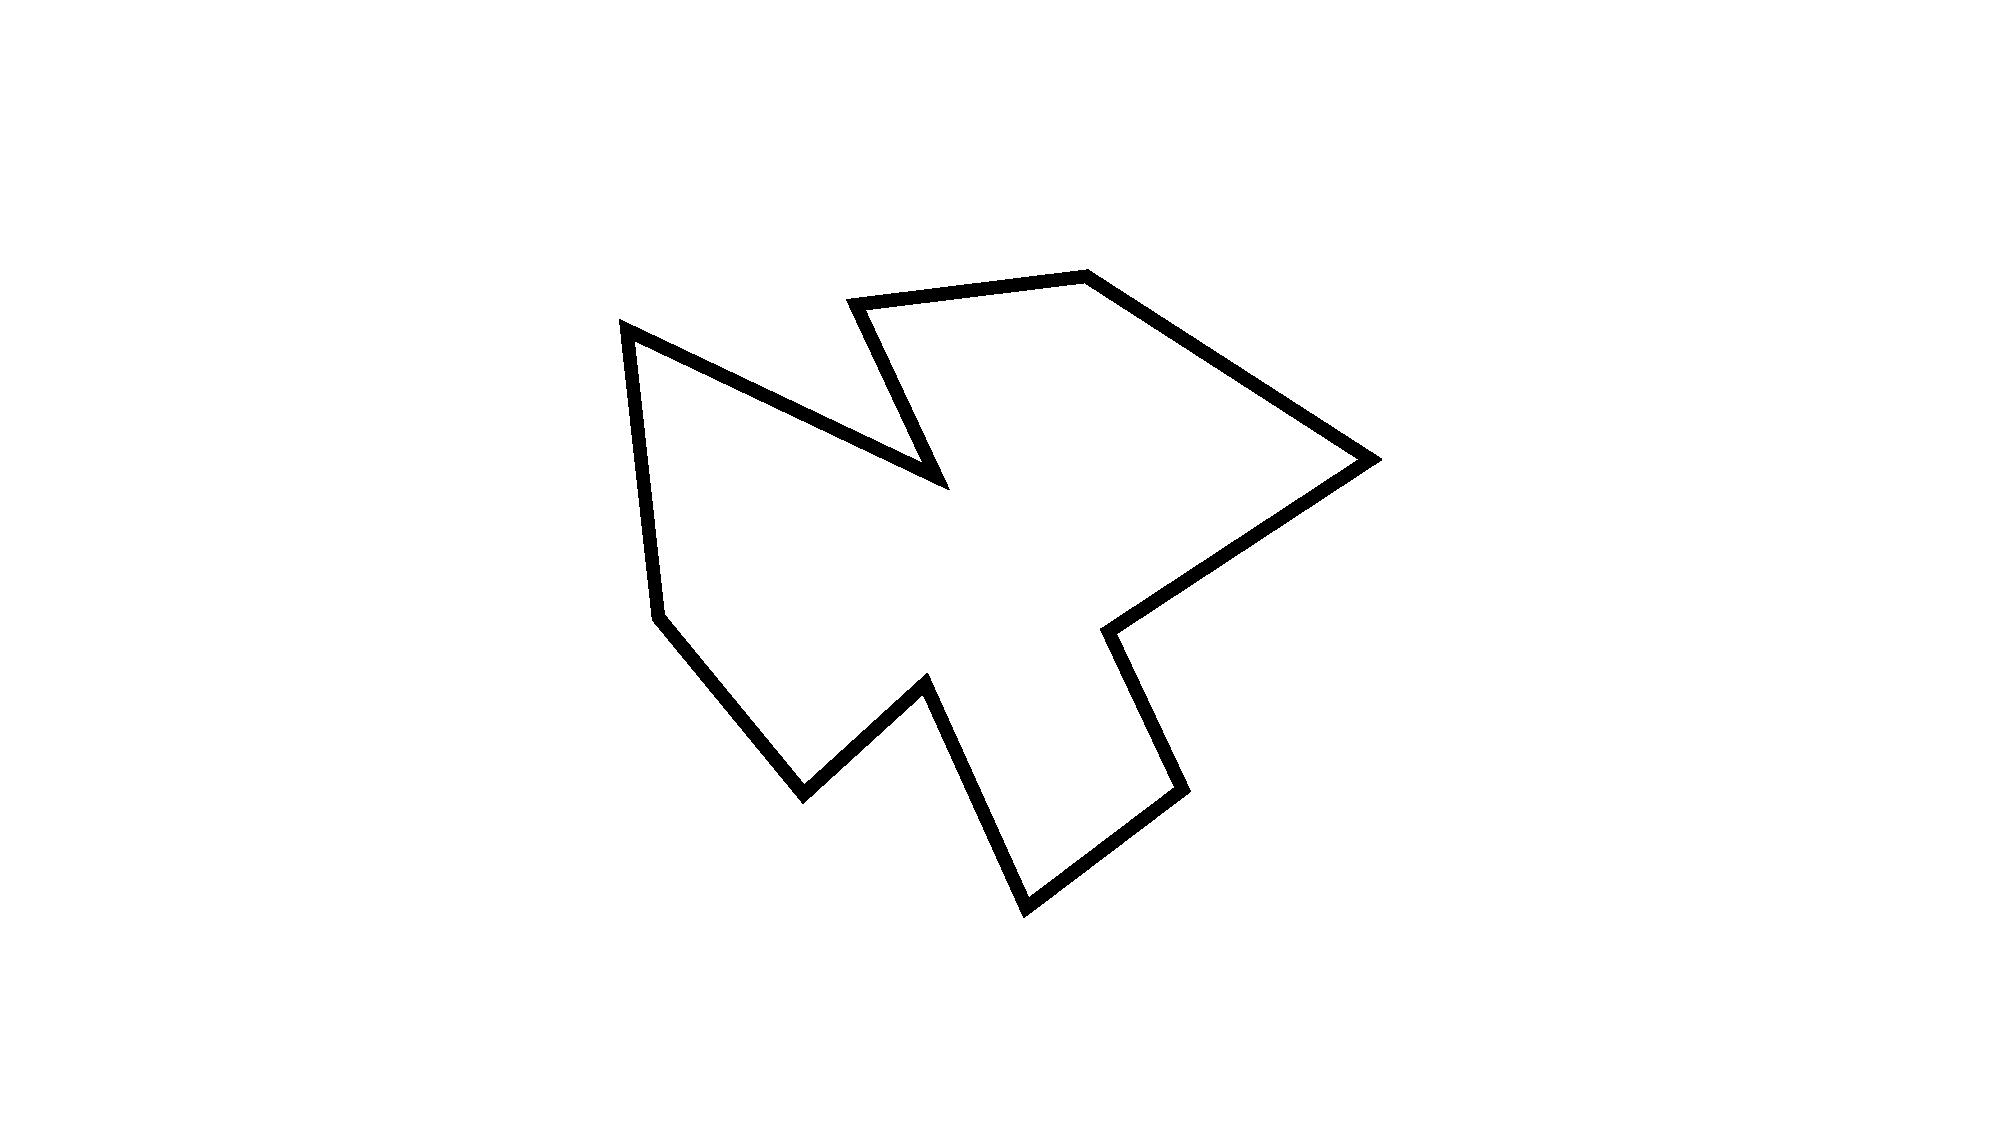
\includegraphics[width=5cm]{../images/worksheet2a.pdf}
\end{center}

\begin{itemize}
\item Is the polygon convex? Why or why not?
\end{itemize}



\item Given the 2 convex polygons, $A$ and $B$, show the steps of the $O(M+N)$ algorithm to find $A \cap B$ discussed in class. Your algorithm should start at $a_0$ and $b_0$. 


\begin{center}
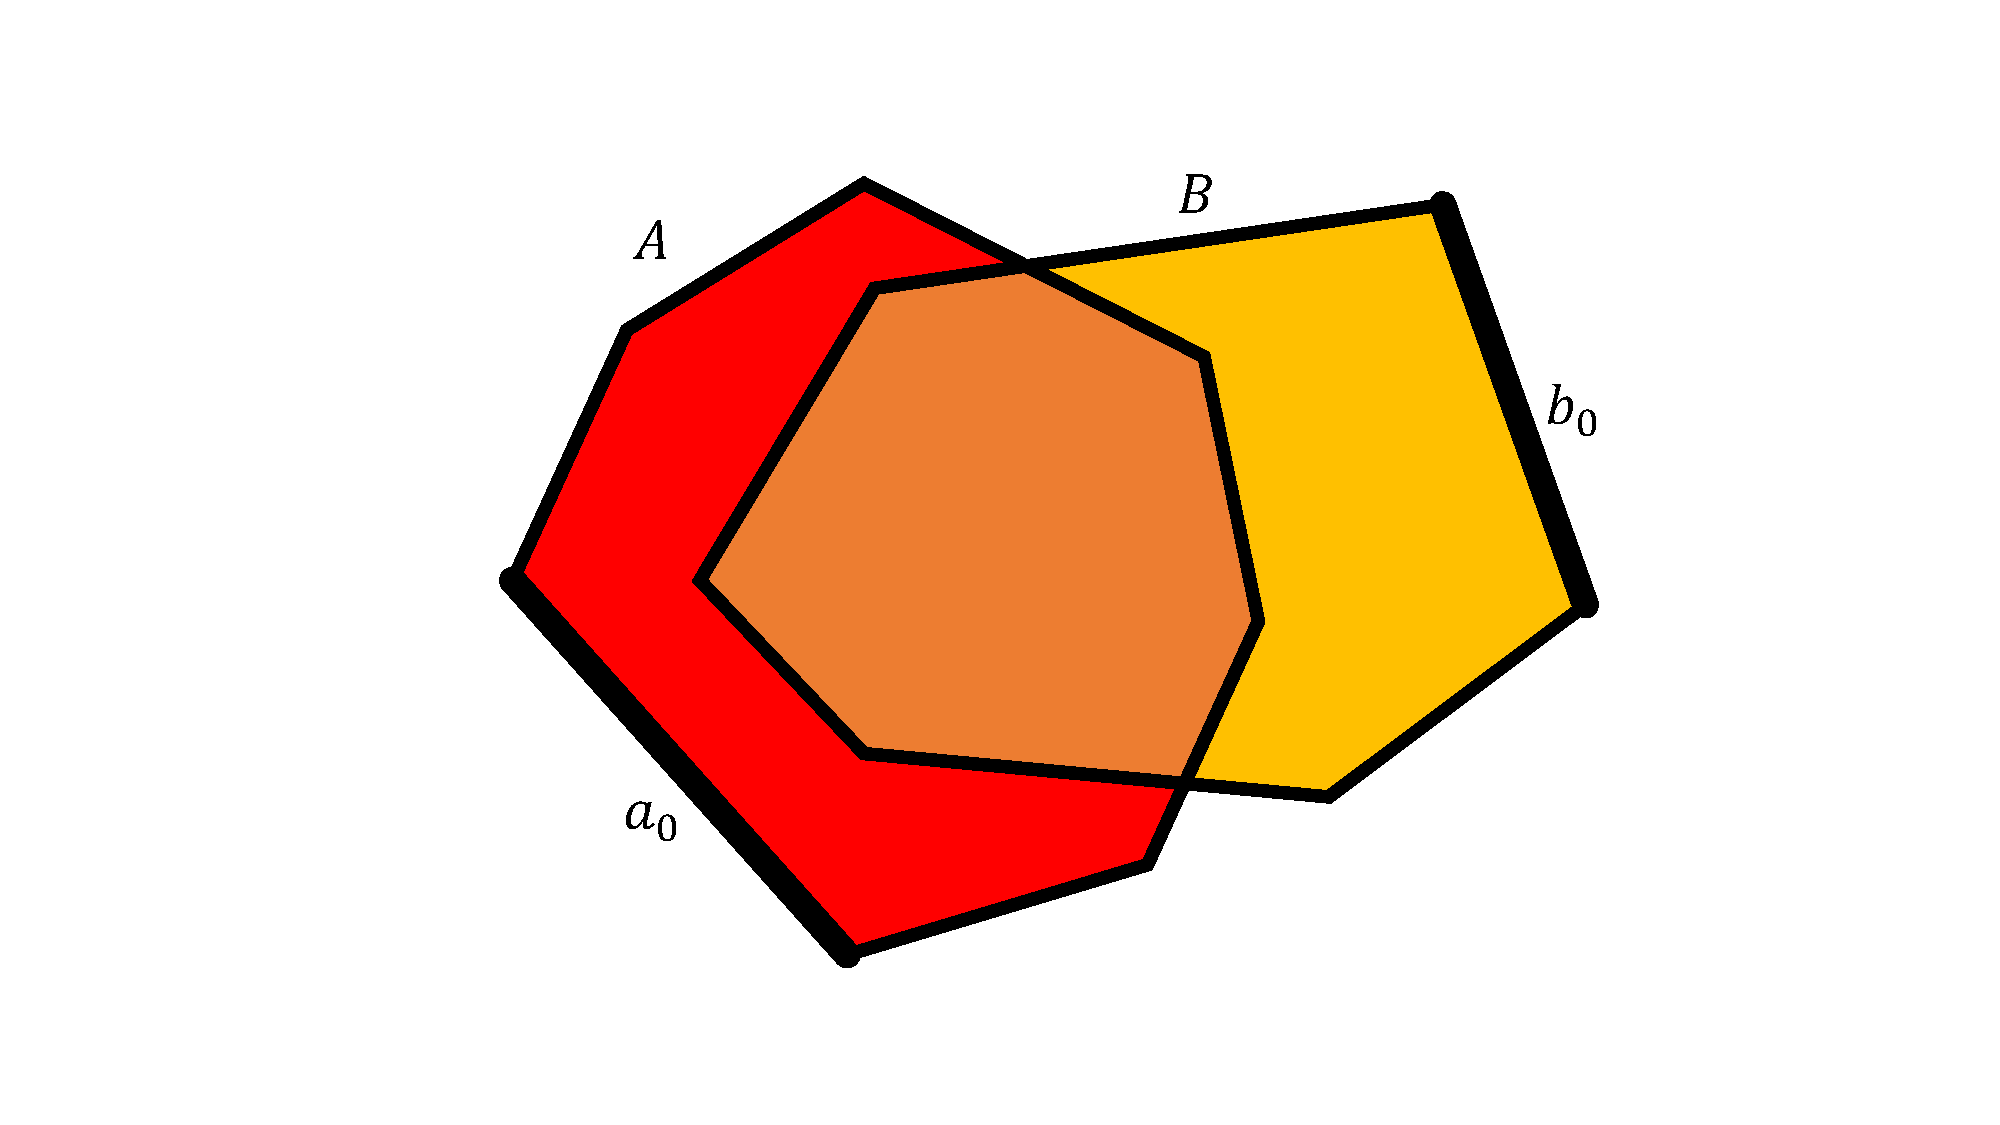
\includegraphics[width=5cm]{../images/worksheet2b.pdf}
\end{center}

\begin{itemize}
\item Describe how you would modify the algorithm to find $A \cup B$, $A \backslash B$, and $A \ominus B$. (hint: describe it in terms of inner and outer chains.)
\end{itemize}


\end{enumerate}


\section{Submission}

\myparagraph{Upload your answers and associated work to canvas as a single scanned, types, or photographed PDF document. Be sure that your submission is legible.}



\end{document}

